		\begin{objectives}
			In this tutorial you will explore some modelling towards optimization problems and using the techniques we have learned to analyze the results.

				These problems relate to the following course learning objectives:
				\begin{itemize}\it 
					\item Model with ODEs. \\[-20pt]
					\item Use Jupyter Notebook to approximate the solution. \\[-20pt]
					\item Create a visualization of the problem and the solution.
				\end{itemize}
%						\textit{Apply linear algebra techniques to classify solutions of linear systems of ordinary differential
%			equations including rigorously classifying the stability of equilibrium solutions and creating
%			linear approximations to non-linear systems of ordinary differential equations.}
		\end{objectives}

\vspace{-.5em}
\subsection*{Problems}
\vspace{-.5em}


\begin{enumerate}
	\item\label{q1} A bee goes from flower to flower to get pollen.
	
	At some point it has to decide when it advantageous to move to a different flower.
	
	Assume the following:
	\begin{itemize}
		\item Let $t$ be the time in minutes since the bee landed in the current flower.
		\item When the bee settles into a flower, it is full of pollen.
		\item The bee starts gathering its pollen at a rate proportional to the amount of pollen left in the flower (with proportionality constant 1).
		\item It takes 1 minute for the bee to find a new flower full of pollen.
	\end{itemize}
	
	\begin{enumerate}
		\item Find a function for the amount of pollen the bee has gathered since it landed on a flower.

		\textbf{Hint. } Keep track of the fraction of pollen still in the flower.
		


		\item Calculate the average rate of pollen gathering by the bee starting from the time the bee left the previous flower until time $t$.



		\item The bee decides to move on to the next flower when the average rate of pollen gathering starts decreasing. At what time does that happen?

		
%		\item Observe that at first the bee collects pollen rapidly, but it starts collecting pollen slower and slower.
%		
%		At some point, the rate at which the bee is collecting pollen becomes smaller than the average rate since it left the previous flower.
%		
%		That is the moment the bee decides to leave the flower to find another one still full of pollen.
%		
%		What is that time $t^\star$?
		

	\item Consider the following figure
	\begin{center}
		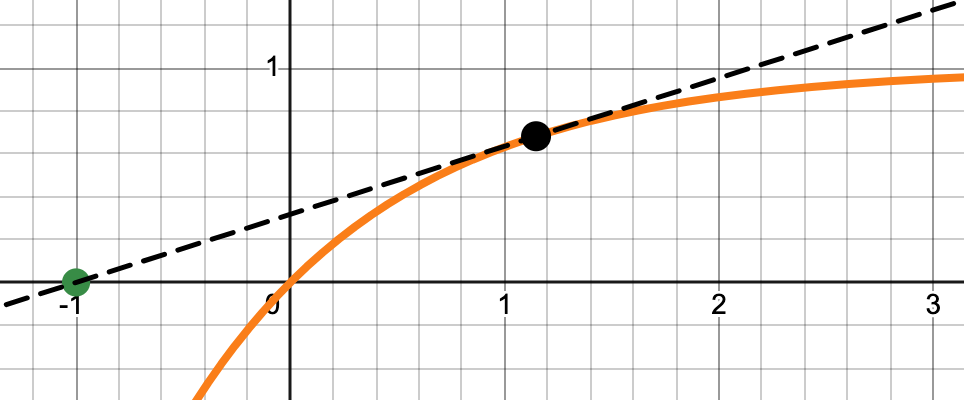
\includegraphics[width=.5\textwidth]{bees.png}
			% https://www.desmos.com/calculator/muodwklknf
	\end{center}
	
	Explain how it relates to this problem.

	\end{enumerate}
	
	

\newpage

\item \label{q2} Let us find a formula for the air density $\rho(y)$ at an altitude of $y$ metres.

\begin{enumerate}

	\item Consider the following two premises:
	\begin{itemize}
		\item[($P_1$)] Air density $\rho$ (in kg/m$^3$) is proportional to air pressure $p$ (in Pa), with proportionality constant $\frac{M}{RT}$, where:
		\begin{itemize}
			\item $M = $ molar mass of dry air $= 0.0289644$ kg/mol
			\item $R = $ ideal gas constant $= 8.31447$ J/(mol$\cdot$K)
			\item $T = $ temperature of the air (assuming it is constant)
		\end{itemize}
		\item[($P_2$)] Air pressure $p$ is the weight of the air above
	\end{itemize}
	
	For each premise, find a relation the air density with the air pressure.
	
	
	\item Using these two relations, obtain an equation for the air density $\rho(y)$. Then obtain a differential equation for the air density $\rho(y)$.
	
	
	\item Solve this differential equation to obtain a formula for the air density $\rho(y)$ assuming that $\rho(y_0) = \rho_0$.
	
	
	\item Use this formula to calculate the mass of Earth's atmosphere.
	
	\begin{minipage}{.7\textwidth}
	Here are some (simplified) facts that will help you:
	\begin{itemize}
		\item The \textbf{troposphere} and \textbf{stratosphere} contain 99.9\% of the mass of the atmosphere\\
	
%	Troposhpere facts:
		\item The temperature in the \textbf{troposphere} decreases linearly with altitude and
		\begin{itemize}
			\item $T_0=$ standard temperature at sea level $=288.15$ K
			\item $L=$ temperature lapse $ = 0.0065$ K/m
		\end{itemize}
		\item Air pressure in the \textbf{troposphere} is given by
			\[ p_T(h) = 	p_0 \left( 1 - \frac{Lh}{T_0} \right)^{\frac{gM}{RL}}\]
			where $h=$ altitude above sea level and $p_0=$ is the standard air pressure at sea level $= 101.325$ kPa \\
	
%	Stratosphere facts:
		\item The temperature in the \textbf{stratosphere} is constant.
	\end{itemize}
	\end{minipage}
	\hfill
	\begin{minipage}{.3\textwidth}
		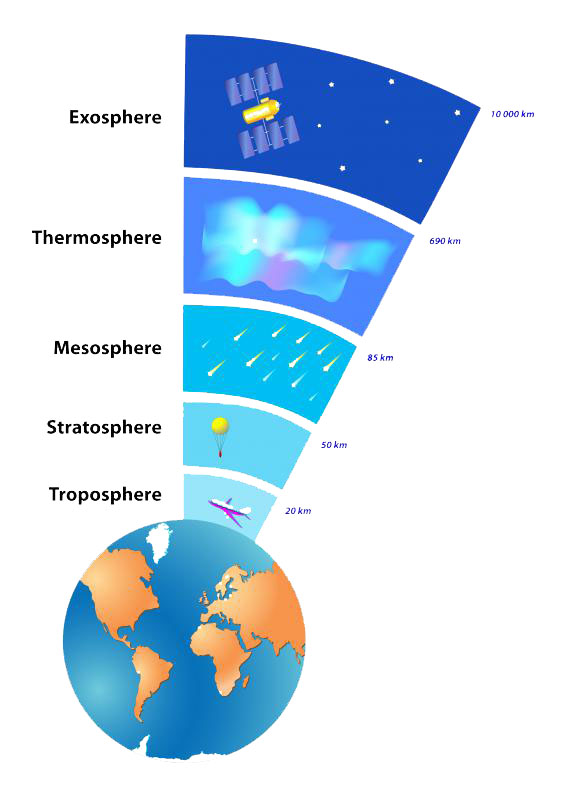
\includegraphics[width=\textwidth]{atmosphere.jpg}
	\end{minipage}

	\item It is often said that the Toposphere contains three quarters of the atmosphere's mass. Using the International Standard Atmosphere\footnote{\url{https://en.wikipedia.org/wiki/International_Standard_Atmosphere}}, check whether this model satisfies this.
	
	\item Compare this to the actual mass of the atmosphere. How can it be improved?

	
\end{enumerate}


	
	
	
	
\end{enumerate}

















